\documentclass{standalone}
\usepackage{tikz}
\usetikzlibrary{patterns, positioning}


\begin{document}
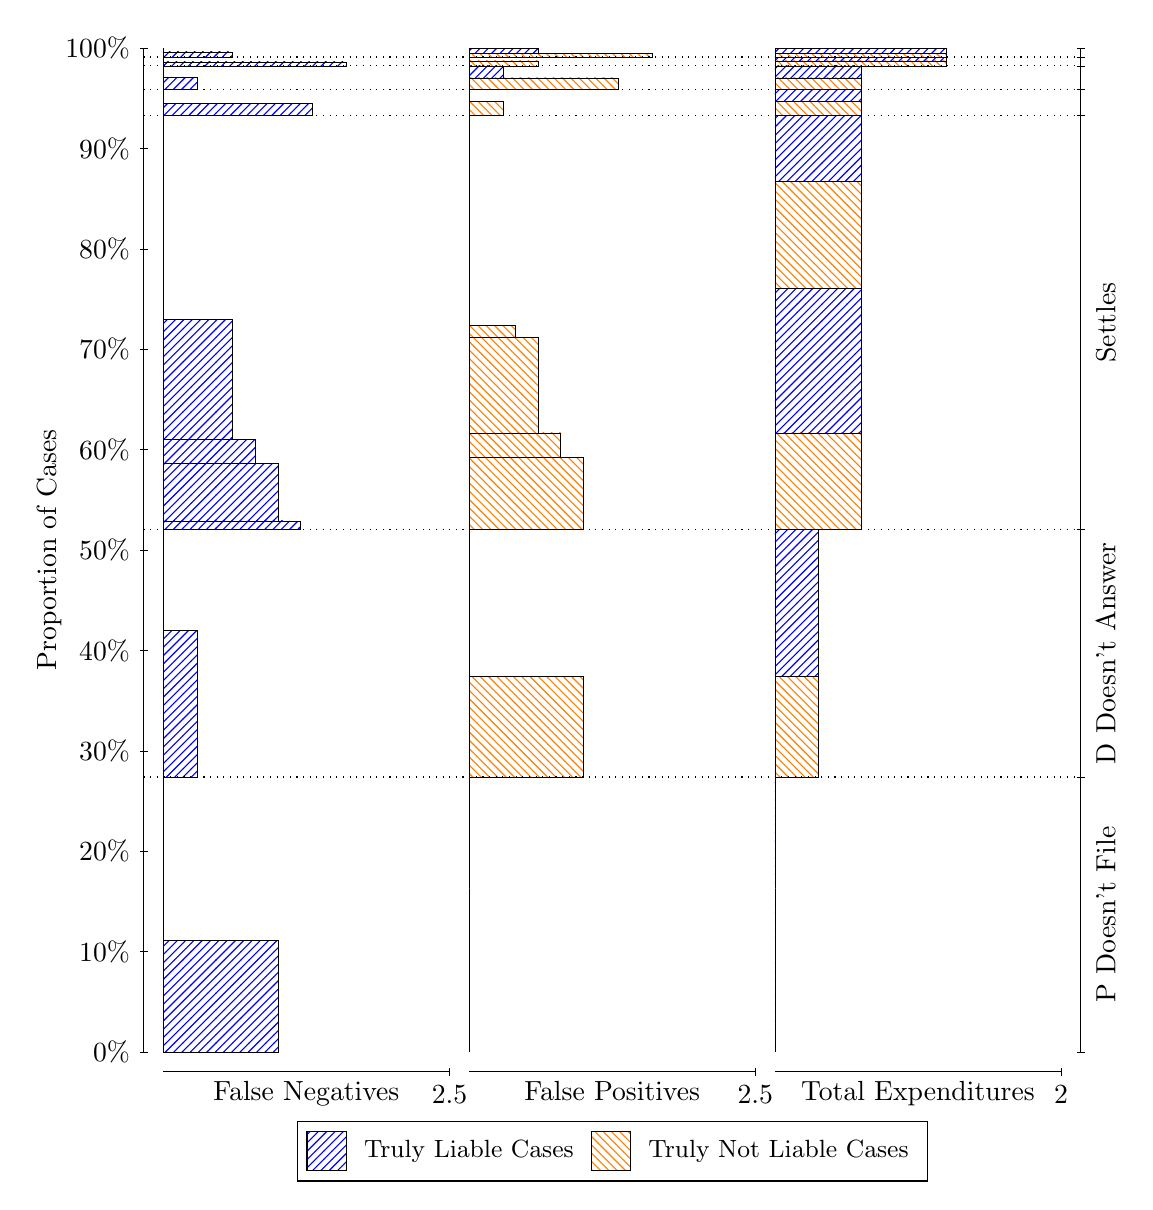
\begin{tikzpicture}
\draw[black, very thin] (1.5,1.75) -- (1.5,14.5);
\node[rotate=90, text=black, anchor=center] at (0.3, 8.125) {Proportion of Cases};
\draw[black, very thin] (1.45,1.75) -- (1.55,1.75);
\node[text=black, anchor=east] at (1.45, 1.75) {0\%};
\draw[black, very thin] (1.45,3.025) -- (1.55,3.025);
\node[text=black, anchor=east] at (1.45, 3.025) {10\%};
\draw[black, very thin] (1.45,4.3) -- (1.55,4.3);
\node[text=black, anchor=east] at (1.45, 4.3) {20\%};
\draw[black, very thin] (1.45,5.575) -- (1.55,5.575);
\node[text=black, anchor=east] at (1.45, 5.575) {30\%};
\draw[black, very thin] (1.45,6.85) -- (1.55,6.85);
\node[text=black, anchor=east] at (1.45, 6.85) {40\%};
\draw[black, very thin] (1.45,8.125) -- (1.55,8.125);
\node[text=black, anchor=east] at (1.45, 8.125) {50\%};
\draw[black, very thin] (1.45,9.4) -- (1.55,9.4);
\node[text=black, anchor=east] at (1.45, 9.4) {60\%};
\draw[black, very thin] (1.45,10.675) -- (1.55,10.675);
\node[text=black, anchor=east] at (1.45, 10.675) {70\%};
\draw[black, very thin] (1.45,11.95) -- (1.55,11.95);
\node[text=black, anchor=east] at (1.45, 11.95) {80\%};
\draw[black, very thin] (1.45,13.225) -- (1.55,13.225);
\node[text=black, anchor=east] at (1.45, 13.225) {90\%};
\draw[black, very thin] (1.45,14.5) -- (1.55,14.5);
\node[text=black, anchor=east] at (1.45, 14.5) {100\%};

\draw[black, very thin] (13.4,1.75) -- (13.4,14.5);
\draw[black, very thin] (13.35,1.75) -- (13.45,1.75);
\node[anchor=west] at (13.35, 1.75) {};
\draw[black, very thin] (13.35,5.2415) -- (13.45,5.2415);
\node[anchor=west] at (13.35, 5.2415) {};
\draw[black, very thin] (13.35,8.3867) -- (13.45,8.3867);
\node[anchor=west] at (13.35, 8.3867) {};
\draw[black, very thin] (13.35,13.644) -- (13.45,13.644);
\node[anchor=west] at (13.35, 13.644) {};
\draw[black, very thin] (13.35,13.975) -- (13.45,13.975);
\node[anchor=west] at (13.35, 13.975) {};
\draw[black, very thin] (13.35,14.273) -- (13.45,14.273);
\node[anchor=west] at (13.35, 14.273) {};
\draw[black, very thin] (13.35,14.386) -- (13.45,14.386);
\node[anchor=west] at (13.35, 14.386) {};
\draw[black, very thin] (13.35,14.5) -- (13.45,14.5);
\node[anchor=west] at (13.35, 14.5) {};

\draw[black, very thin, pattern color=blue, pattern=north east lines] (1.75,1.75) rectangle (3.2033,3.1665);
\draw[black, very thin, pattern color=orange, pattern=north west lines] (1.75,3.1665) rectangle (1.75,5.2415);
\draw[black, very thin, pattern color=blue, pattern=north east lines] (1.75,5.2415) rectangle (2.186,7.1068);
\draw[black, very thin, pattern color=orange, pattern=north west lines] (1.75,7.1068) rectangle (1.75,8.3867);
\draw[black, very thin, pattern color=blue, pattern=north east lines] (1.75,8.3867) rectangle (3.494,8.4908);
\draw[black, very thin, pattern color=blue, pattern=north east lines] (1.75,8.4908) rectangle (3.3487,8.4934);
\draw[black, very thin, pattern color=blue, pattern=north east lines] (1.75,8.4934) rectangle (3.2033,9.2209);
\draw[black, very thin, pattern color=blue, pattern=north east lines] (1.75,9.2209) rectangle (2.9127,9.5324);
\draw[black, very thin, pattern color=blue, pattern=north east lines] (1.75,9.5324) rectangle (2.622,11.056);
\draw[black, very thin, pattern color=orange, pattern=north west lines] (1.75,11.056) rectangle (1.75,13.644);
\draw[black, very thin, pattern color=blue, pattern=north east lines] (1.75,13.644) rectangle (3.6393,13.801);
\draw[black, very thin, pattern color=orange, pattern=north west lines] (1.75,13.801) rectangle (1.75,13.975);
\draw[black, very thin, pattern color=blue, pattern=north east lines] (1.75,13.975) rectangle (2.186,14.129);
\draw[black, very thin, pattern color=orange, pattern=north west lines] (1.75,14.129) rectangle (1.75,14.273);
\draw[black, very thin, pattern color=blue, pattern=north east lines] (1.75,14.273) rectangle (4.0753,14.323);
\draw[black, very thin, pattern color=orange, pattern=north west lines] (1.75,14.323) rectangle (1.75,14.386);
\draw[black, very thin, pattern color=blue, pattern=north east lines] (1.75,14.386) rectangle (2.622,14.45);
\draw[black, very thin, pattern color=orange, pattern=north west lines] (1.75,14.45) rectangle (1.75,14.5);
\draw[black, very thin, pattern color=orange, pattern=north west lines] (5.6333,1.75) rectangle (5.6333,3.825);
\draw[black, very thin, pattern color=blue, pattern=north east lines] (5.6333,3.825) rectangle (5.6333,5.2415);
\draw[black, very thin, pattern color=orange, pattern=north west lines] (5.6333,5.2415) rectangle (7.0867,6.5214);
\draw[black, very thin, pattern color=blue, pattern=north east lines] (5.6333,6.5214) rectangle (5.6333,8.3867);
\draw[black, very thin, pattern color=orange, pattern=north west lines] (5.6333,8.3867) rectangle (7.0867,9.3004);
\draw[black, very thin, pattern color=orange, pattern=north west lines] (5.6333,9.3004) rectangle (6.796,9.612);
\draw[black, very thin, pattern color=orange, pattern=north west lines] (5.6333,9.612) rectangle (6.5053,10.826);
\draw[black, very thin, pattern color=orange, pattern=north west lines] (5.6333,10.826) rectangle (6.36,10.829);
\draw[black, very thin, pattern color=orange, pattern=north west lines] (5.6333,10.829) rectangle (6.2147,10.975);
\draw[black, very thin, pattern color=blue, pattern=north east lines] (5.6333,10.975) rectangle (5.6333,13.644);
\draw[black, very thin, pattern color=orange, pattern=north west lines] (5.6333,13.644) rectangle (6.0693,13.818);
\draw[black, very thin, pattern color=blue, pattern=north east lines] (5.6333,13.818) rectangle (5.6333,13.975);
\draw[black, very thin, pattern color=orange, pattern=north west lines] (5.6333,13.975) rectangle (7.5227,14.12);
\draw[black, very thin, pattern color=blue, pattern=north east lines] (5.6333,14.12) rectangle (6.0693,14.273);
\draw[black, very thin, pattern color=orange, pattern=north west lines] (5.6333,14.273) rectangle (6.5053,14.336);
\draw[black, very thin, pattern color=blue, pattern=north east lines] (5.6333,14.336) rectangle (5.6333,14.386);
\draw[black, very thin, pattern color=orange, pattern=north west lines] (5.6333,14.386) rectangle (7.9587,14.436);
\draw[black, very thin, pattern color=blue, pattern=north east lines] (5.6333,14.436) rectangle (6.5053,14.5);
\draw[black, very thin, pattern color=orange, pattern=north west lines] (9.5167,1.75) rectangle (9.5167,3.825);
\draw[black, very thin, pattern color=blue, pattern=north east lines] (9.5167,3.825) rectangle (9.5167,5.2415);
\draw[black, very thin, pattern color=orange, pattern=north west lines] (9.5167,5.2415) rectangle (10.062,6.5214);
\draw[black, very thin, pattern color=blue, pattern=north east lines] (9.5167,6.5214) rectangle (10.062,8.3867);
\draw[black, very thin, pattern color=orange, pattern=north west lines] (9.5167,8.3867) rectangle (10.607,9.612);
\draw[black, very thin, pattern color=blue, pattern=north east lines] (9.5167,9.612) rectangle (10.607,11.447);
\draw[black, very thin, pattern color=orange, pattern=north west lines] (9.5167,11.447) rectangle (10.607,12.809);
\draw[black, very thin, pattern color=blue, pattern=north east lines] (9.5167,12.809) rectangle (10.607,13.644);
\draw[black, very thin, pattern color=orange, pattern=north west lines] (9.5167,13.644) rectangle (10.607,13.818);
\draw[black, very thin, pattern color=blue, pattern=north east lines] (9.5167,13.818) rectangle (10.607,13.975);
\draw[black, very thin, pattern color=orange, pattern=north west lines] (9.5167,13.975) rectangle (10.607,14.12);
\draw[black, very thin, pattern color=blue, pattern=north east lines] (9.5167,14.12) rectangle (10.607,14.273);
\draw[black, very thin, pattern color=orange, pattern=north west lines] (9.5167,14.273) rectangle (11.697,14.336);
\draw[black, very thin, pattern color=blue, pattern=north east lines] (9.5167,14.336) rectangle (11.697,14.386);
\draw[black, very thin, pattern color=orange, pattern=north west lines] (9.5167,14.386) rectangle (11.697,14.436);
\draw[black, very thin, pattern color=blue, pattern=north east lines] (9.5167,14.436) rectangle (11.697,14.5);
\draw[black, dotted] (1.5,5.2415) -- (13.4,5.2415);
\draw[black, dotted] (1.5,8.3867) -- (13.4,8.3867);
\draw[black, dotted] (1.5,13.644) -- (13.4,13.644);
\draw[black, dotted] (1.5,13.975) -- (13.4,13.975);
\draw[black, dotted] (1.5,14.273) -- (13.4,14.273);
\draw[black, dotted] (1.5,14.386) -- (13.4,14.386);
\draw[black, very thin] (1.75,1.5) -- (5.3833,1.5);
\node[text=black, anchor=north] at (3.5667, 1.5) {False Negatives};
\draw[black, very thin] (5.3833,1.45) -- (5.3833,1.55);
\node[text=black, anchor=north] at (5.3833, 1.45) {2.5};

\draw[black, very thin] (5.6333,1.5) -- (9.2667,1.5);
\node[text=black, anchor=north] at (7.45, 1.5) {False Positives};
\draw[black, very thin] (9.2667,1.45) -- (9.2667,1.55);
\node[text=black, anchor=north] at (9.2667, 1.45) {2.5};

\draw[black, very thin] (9.5167,1.5) -- (13.15,1.5);
\node[text=black, anchor=north] at (11.333, 1.5) {Total Expenditures};
\draw[black, very thin] (13.15,1.45) -- (13.15,1.55);
\node[text=black, anchor=north] at (13.15, 1.45) {2};

\node[text=black, centered, rotate=90] at (13.72, 3.4958) {P Doesn't File};
\node[text=black, centered, rotate=90] at (13.72, 6.8141) {D Doesn't Answer};
\node[text=black, centered, rotate=90] at (13.72, 11.015) {Settles};





\draw (7.449999999999999,1.5) node[draw=none] (baseCoordinate) {};
\begin{scope}[align=center]
        \matrix[scale=0.5, draw=black, below=0.5cm of baseCoordinate, nodes={draw}, column sep=0.1cm]{
            \node[rectangle, draw, minimum width=0.5cm, minimum height=0.5cm, pattern color=blue, pattern=north east lines] {}; &
            \node[draw=none, font=\small, text=black] (B) {Truly Liable Cases}; &
            \node[rectangle, draw, minimum width=0.5cm, minimum height=0.5cm, pattern color=orange, pattern=north west lines] {}; &
            \node[draw=none, font=\small, text=black] (B) {Truly Not Liable Cases}; \\
            };
\end{scope}

\end{tikzpicture}
\end{document}